\documentclass[12pt]{scrartcl}

\usepackage[T1]{fontenc}
\usepackage[utf8]{inputenc}

\usepackage{amstext}
\usepackage{color}
\usepackage{dcolumn}
   \newcolumntype{d}[1]{D{.}{.}{#1}}
\usepackage{dsfont}
\usepackage{float}
\usepackage{geometry}
   \geometry{verbose,tmargin=1.4in,bmargin=1.4in,lmargin=1.4in,rmargin=1.4in}
\usepackage{graphicx}
\usepackage[hidelinks]{hyperref}
   \urlstyle{same}
\usepackage{lscape}
\usepackage[authoryear]{natbib}
\usepackage{setspace}

\deffootnote{1.5em}{1em}{\makebox[1.5em][l]{\thefootnotemark}}
   \setlength{\skip\footins}{1.5em}
   \setlength{\footnotesep}{1em}

\addtokomafont{disposition}{\rmfamily}

\begin{document}
\thispagestyle{empty}
\renewcommand{\thefootnote}{\fnsymbol{footnote}}
\begin{center}
{\LARGE Thinking About Need}\\\vspace{2ex}
{\Large A Vignette Experiment}\\\vspace{6ex}
{\large Alexander Max Bauer,$^a$\footnotemark[1] Adele Diederich,$^b$\\Stefan Traub,$^{c}$ Arne Weiß$^d$}\\\vspace{3ex}
\textsl{\small $^{a}$Dept. of Philosophy, University of Oldenburg, Oldenburg, Germany}\\\vspace{1ex}
\textsl{\small $^{b}$Dept. of Psychology \& Methods, Constructor University, Bremen, Germany}\\\vspace{1ex}
\textsl{\small $^{c}$Dept. of Economics, Helmut-Schmidt-University, Hamburg, Germany}\\\vspace{1ex}
\textsl{\small $^{d}$Dept. of Economics, University of Alicante, Alicante, Spain}\\\vspace{3ex}
April 25, 2023
\end{center}

\vspace{\fill}

\noindent\textbf{Abstract:} We examine the role of need satisfaction in non-comparative justice ratings about endowments with goods. 
As normative approaches, we discuss utilitarianism, prioritarianism, and sufficientarianism.
Using a vignette experiment, we show that need increases prioritarianistic and sufficientarianistic justice ratings, which leads to an ethically problematic sigmoid shape of the justice evaluation function.
\\[2ex]
\noindent\textbf{Keywords:} Basic Needs, Justice Principles, Prioritarianism, Sufficientarianism, Utilitarianism, Vignette Experiment\\[2ex]
\textbf{JEL Classification:} I30, D63, D31

\footnotetext[1]{Corresponding author.
Department of Philosophy, University of Oldenburg, Ammerl{\"a}nder Heerstra{\ss}e 114--118, 26129 Oldenburg, Germany, \href{mailto:alexander.max.bauer@uni-oldenburg.de}{alexander.max.bauer@uni-oldenburg.de}.
Telephone: +49 (0)441 798 2034.
Financial support by the German Research Foundation (DFG Grants SI $1731/2-2$, TR $458/6-2$) is gratefully acknowledged.
We are indebted to the support and input throughout all project phases by Jan Romann, Nils Springhorn, and Mark Siebel.
We also thank James Konow, Jakob Koscholke, Michael Schippers, Thomas Schramme, and Kai Spiekermann, as well as participants at DFG Research Group 2104 meetings for helpful discussions.}
\renewcommand{\thefootnote}{\arabic{footnote}}\setcounter{footnote}{0}
\newpage


%%%%%%%%%%%%%%%%
% INTRODUCTION %
%%%%%%%%%%%%%%%%
\section{Introduction}\label{sec:introduction}
How do laypersons evaluate the justice of personal endowments with goods that satisfy basic needs?
\cite{miller_principles_1999} emphasizes that needs are not to be confused with wants; they rely on a socially shared notion.
Need, then, refers to whether someone has \textit{enough} \citep{frankfurt_inequality_2015} to live a \textit{decent life} \citep{miller_principles_1999}.
The question of whether someone has enough or not points to the \textit{non-comparative} \citep{feinberg_noncomparative_1974} thrust of need as a criterion of justice: It is human suffering due to unfulfilled needs that causes injustice, not how one is treated relative to others.
This raises the question of how justice is related to need satisfaction, to which the literature offers no precise answer.
In this paper, we first discuss the non-comparative dimension of need-based justice using three normative approaches: utilitarianism \citep[e.\,g.,][]{bentham_introduction_2009,mill_utilitarianism_1998}, prioritarianism \citep[e.\,g.,][]{parfit_equality_1997}, and sufficientarianism \citep[e.\,g.,][]{frankfurt_equality_1987,crisp_egalitarianism_2003,schramme_is_2006}.
We then present an empirical investigation of justice ratings of laypersons using a vignette experiment.

In the vignette experiment, we asked subjects to rate different endowments with living space in terms of justice.
An explicit need threshold was communicated in a need treatment, which was absent in a control treatment.
Additionally, there were two different ratings tasks.
In the global rating task, 11 scenarios of endowment with living space had to be rated individually.
In the relative rating task, pairs of scenarios had to be evaluated in comparison to each other.
The absolute rating task is comparable in procedure and interpretation to the ``method of constant stimuli'' known from psychometrics.
We estimate a justice evaluation function (JEF) from the justice ratings of the subjects using a Weibull function \citep{wichmann_psychometric_2001,mortensen_additive_2002}, which describes the probability that subjects evaluate the stimulus as exceeding the comparison stimulus \citep[p.~2503]{treutwein_adaptive_1995}.
Accordingly, the average justice rating derived from the JEF can be interpreted as the probability that society perceives a given endowment with living space as just.

Vignette experiments have become the de facto methodological standard for empirical justice research because they promise both experimental control about predictor variables (in our case: need satisfaction) and external validity for situations that, for ethical or practical reasons, can not be studied in real-life situations (see \citealp{bardsley_experimental_2009}; for overviews see \citealp{traub_friedman_2005,gaertner_empirical_2012}).
This clearly applies to research on human needs.
While this paper is not the first to empirically study the role of needs for justice evaluations (starting with \citealp{yaari_dividing_1984}, for an overview see \citep[see][]{traub_need-based_2020}, we are not aware of any empirical work, nor a conceptual framework for that matter, that can shed light on the precise relationship between need satisfaction and justice ratings.

Our main results are as follows: The analysis of the absolute average justice ratings shows that an exogenous need threshold for endowment with living space leads to a \textit{sigmoid} JEF.
Below the need threshold, the JEF is convex and justice ratings are lower than without a need threshold.
If the endowment with living space is at least as high as the need threshold, the JEF is concave and the ratings close to the need threshold are significantly above the ratings without need threshold.
This rating pattern is confirmed by the analysis of the relative justice ratings.
The analysis of the individual justice ratings shows that a large proportion of the subjects can be assigned to one of the three justice types: sufficientarianism, prioritarianism, or utilitarianism.
The treatment with a need threshold significantly shifts justice ratings in favor of sufficientariansm and prioritarianism.

Our vignette experiment, therefore, contributes to answering the question of how laypersons think about need.
In our setting, where the focus is on the non-comparative dimension of justice ratings, need significantly changes both individual and average justice ratings.
However, the convexity of the JEF below the need threshold, caused primarily by increases in sufficientarianistic and prioritarianistic justice ratings, also raises ethical problems.
For example, the impression of greater overall justice may be generated by helping those who have only slightly less than the need threshold than by helping those who have the least.

The remainder of the paper is organized as follows.
In the next section, we provide a review of the relevant literature.
In Subsection \ref{sec:need}, we first focus on the concept of need.
In Subsection \ref{sec:principles}, we relate need to various non-comparative principles of justice.
The design of our vignette experiment is presented in Section \ref{sec:experiment}.
In Subsection \ref{sec:treatments}, we begin by explaining the subjects' decision task.
Subsection \ref{sec:remarks} classifies our approach methodologically.
In the third subsection, we formulate expectations for the subjects' decision behavior.
Subsection \ref{sec:procedure} contains details on the execution of the experiment.
The results of the experiment are presented in Section \ref{sec:results}.
We start in Subsection \ref{sec:global} with the mean justice ratings in the global rating task.
Subsection \ref{sec:relative} shows the mean justice ratings in the relative rating task.
The individual justice ratings are analyzed in Subsection \ref{sec:individual}.
The paper ends with a summary and discussion of the results in Section \ref{sec:conclusion}.


%%%%%%%%%%%%%%
% LITERATURE %
%%%%%%%%%%%%%%
\section{Literature Review}\label{sec:background}


%%%%%%%%
% NEED %
%%%%%%%%
\subsection{The Concept of Need}\label{sec:need}
Needs influence our thinking in many areas.
Take, for example, social policy.
Here, one might think of minimum wages or---especially---of \textit{means-tested benefits}, which are an essential element of the liberal (i.\,e., mostly Anglo-Saxon) ``World of Welfare Capitalism'' \citep{esping-andersen_three_1990}.
Means-tested benefits stand in the tradition of the ``poor laws'' that differentiated between deserving and undeserving poor.
This distinction---in itself already a separation between the needy and the not-needy---lives on, for example, in the United States welfare system.
Here, only those who fulfill certain criteria, such as the presence of a disability or a pregnancy, are eligible for benefits from the governmental health program ``Medicaid''---but only if they also have an insufficient income under a poverty threshold which was initially defined by congress as a triple of the amount needed for basic nutrition in the year 1963 and is adjusted for inflation annually.
This poverty threshold can be seen as a collectively determined concept of basic need, which serves as a guideline for social policy.

This is also the case for the ``applicable amount'' defined by the government of the United Kingdom, which was (and still is, in the case of the ``Universal Credit'' program) the reference point for the government's old welfare programs.
In conservative, rather contribution-based welfare states like Germany, need also plays a crucial role in the provision of welfare.
The means-tested and workfare-based unemployment allowance ``Arbeitslosengeld II'' (replaced by the ``B{\"u}rgergeld'' as of 2023) defines a household consisting of family members or mutually dependent residents explicitly as a ``Bedarfs\-gemeinschaft''---a companionship with a shared need.
This need is defined following a statistically assembled consumer basket and adjusted annually following the development of prices and wages.
In like manner, the ``BAf{\"o}G'' (``Federal Law on Support in Education'') defines how much students need for their livelihood.
Corresponding to the central role of the family in the conservative welfare state and its principle of subsidiarity, the student's parents are primarily responsible for providing the student's livelihood.
Only if their income is insufficient will the government fill the resulting gap by granting benefits that consist of equal shares of a grant and an interest-free loan.

The concept of need can also be found when it comes to the assessment of poverty.
Besides the measures of relative and absolute poverty, another poverty indicator that strongly corresponds with the idea of need is the concept of ``material deprivation''.
Here, sets of items are used to evaluate whether an individual can be considered ``materially deprived''.
Those sets vary but include, in many cases, basic needs like the ``ability to adequately heat the dwelling'', the ``ability to have a healthy diet'', the ``ability to clothe properly'', or ``access to health care'' \citep[p.~37]{boarini_measures_2006}.
Needs, therefore, do not only play a role in the formulation of policies but also when it comes to assessing whether there is a necessity for political intervention or when it comes to evaluating if the actions taken were successful.

Besides these practical and evaluative perspectives, need has---as \cite{bauer_need_2022} have pointed out---also been of importance in political theory \citep{dean_translation_2013,doyal_theory_1984,nussbaum_human_1992,weale_political_1984}, has been suggested by many as a fundamental cornerstone for human rights \citep[e.\,g.,][]{brock_needs_2005,gasper_needs_2005,renzo_human_2015}, and has also gained traction in positive justice research \citep[for summary of some recent work, see, e.\,g.,][]{miller_needs-based_2020}.
While early empirical research on distributive justice attitudes in the 1960s and 1970s focused on \textit{equity theory}, this focus changed during the 1970s and 1980s with, for example, \cite{deutsch_equity_1975} arguing that such a singular approach confounds distinct allocation principles.
Instead, he suggested studying equity, equality, and need as different principles.
In a similar manner, \cite{schwinger_just_1980} suggested contribution, equality, and need, \cite{wagstaff_equity_1994} equity, equality, and need, and \cite{konow_fair_2001} equity, efficiency, and need.
As \cite{konow_is_2009} notes, empirical investigations increasingly find preferences for unequal distributions, giving room for principles other than equality.
Concerning need, it is notable that people were found to prefer distributions that comply with securing floor levels \citep[e.\,g.][]{ahlert_thresholds_2012,frohlich_choosing_1992,frohlich_choices_1987}.

But, after all, what \textit{is} a need?
As \cite{bauer_need_2022} have summarized, a need can be defined as a necessity of a good which is required by some person to avoid being harmed.
Such needs can be biological (e.\,g., the need for hydration or nutrition) or social (as in the famous example of the linen shirt by \citealt{smith_wealth_1979}).
Needs are not to be confused with wants; they rely on a socially shared notion \citep{miller_principles_1999}.
An individual may have such a strong preference for eating bluefin tuna that she feels pain whenever it is not part of her menu.
For this want to become a need, however, others must \textit{acknowledge} that eating bluefin tuna is necessary for her not to be harmed (which in this case seems fairly unlikely).
As an inter-subjectively acknowledged threshold, needs provide a fundamentally different basis of social justice than other criteria, such as equality, equity, or the Rawlsian maximin principle.

What sets the need criterion apart from the latter is its defining question: Do people have enough \citep{frankfurt_inequality_2015} to lead a minimally decent life \citep{miller_principles_1999}?
This question shows the \textit{non-comparative} \citep{feinberg_noncomparative_1974} thrust of need-based justice: It is, first of all, human suffering due to unfulfilled needs that causes injustice, not how one is treated relative to others.
This raises the question of how justice is related to need satisfaction, to which the literature offers no precise answer.

The main reason for this gap might lie in the focus of many accounts of social justice on the \textit{comparative} dimension of justice, that is, how one person's due is related to how much other members of society receive.
This is clearly an important endeavor, and a focus on need does not make it obsolete.\footnote{The comparative dimension is always present when members of society differ in important aspects and need considerations stop carrying much weight when everyone's needs are fulfilled.}
However, there seems to have been little progress in reaching common principles of comparative justice accepted by involved parties with their differing interests and their selfishly biased perceptions.

Seeing justice through the lens of need satisfaction, however partial that perspective may be, might have a vital upshot: Since need thresholds are based on a shared understanding within society, need-based justice may have the chance to reach a consensus, even among involved parties, that harm should be avoided, regardless of a suffering person's desert, status, or responsibility.
The relative silence in the literature on the relationship between need satisfaction and justice is therefore an important gap: If all we can say is that unnecessary suffering is unjust, how can we, as theorists or policy-makers, differentiate between situations with \textit{different levels of suffering} or decide between situations that involve trade-offs between members of society?

In this paper, we focus solely on the non-comparative dimension of justice, hitherto largely neglected in both the empirical and the normative literature.\footnote{A comparative measure of need-based justice, which is based on the inequality of unsatisfied need, was developed by \citet{miller_principles_1999}. For a critical discussion, see \citet{siebel_need_2020}. For a more recent comparative measure of need-based justice, see \citet{springhorn_measurement_2022}.}
Against this background, we will present empirical data based on evaluations of subjects acting as \textit{impartial spectators} in a vignette experiment.
As many have argued (see, e.\,g., \citealp{konow_which_2003}, and \citealp{miller_distributive_2017}), the impartial views of real people are a crucial foundation for political and normative theory.
Asking laypersons helps the theorist to go beyond and possibly question her own pre-theoretical intuitions.
Not least, for a theory of justice to be capable of reaching a consensus, it has to be accepted by non-experts \citep[also see][]{bauer_philosophie_2019,bauer_empirical_2020}.


%%%%%%%%%%%%%%
% PRINCIPLES %
%%%%%%%%%%%%%%
\subsection{Principles of Justice and the Justice Evaluation Function}\label{sec:principles}
Now, how is need related to different principles of justice?
It seems a clear point of departure to characterize a situation of unfulfilled needs as less just than a situation in which needs are fulfilled \citep{kipnis_economic_1985}.
This follows straightforwardly from several accounts of justice which acknowledge a non-comparative dimension, such as utilitarianism, prioritarianism, or sufficientarianism (variations of these theories will be coming up again later when we evaluate the individual data of our participants, see Section \ref{sec:individual}).\footnote{It may even be deduced from the writings of Plato and Cicero \citep[see][]{siebel_each_2017}.}
While utilitarianism focuses on the overall outcome \citep[e.\,g.,][]{bentham_introduction_2009,mill_utilitarianism_1998}, prioritarianism puts extra weight on the well-being of those who are particularly ill off \citep[e.\,g.,][]{parfit_equality_1997}, and sufficientarianism strives for everyone to have at least enough \citep[e.\,g.,][]{frankfurt_equality_1987,crisp_egalitarianism_2003,schramme_is_2006}.

Moreover, one may differentiate between \textit{qualitative} and \textit{quantitative} accounts of need-based justice \citep[see][]{siebel_need_2020}.
A purely qualitative principle is `binary' in that---after having identified a need---it simply differentiates between just and unjust endowments without making a statement about how just or unjust the endowment with the respective good or service is.
A quantitative principle additionally makes it possible to measure (and compare) the degree of need-satisfaction, but it involves measurement and scaling issues \citep[see][]{diederich_identifying_2020}.

Suppose that a quantitative measurement of justice that is based on the satisfaction of basic needs exists---a (cardinal, real-valued) \textit{justice evaluation function} (JEF) that is (weakly) monotonic increasing with respect to the endowment.
Then, further questions arise about its properties, particularly regarding its ``behavior'' around the need threshold (i.\,e., the point of complete need satisfaction).
First, precisely how is justice rising below the need threshold (i.\,e., what can be said about the second derivative of the JEF)?
Second, what does the shape of the JEF look like beyond the need threshold?

From the perspective of utilitarianism, justice rises in pleasure and falls in pain; more generally, it increases in a person's utility.
For lack of compelling alternatives, let us assume a proportional relationship between justice and utility on a certain interval, namely the utility arising from the minimum and the maximum possible endowment with the good a person is in need of.
Consequently, the relationship between endowment and utility determines the functional form of the JEF.
The dominant assumption for this relationship is that of diminishing marginal returns.
Putting these elements together suggests a \textit{concave} relation between endowment and justice (i.\,e., the second derivative of the JEF is negative).

The same conclusion could, unsurprisingly, also be drawn from the perspective of prioritarianism, which gives more weight to the utility of those who are badly off.
According to \citet{arneson_egalitarianism_2002}, injustice is directly linked to a person's suffering (and not to the level of inequality), which gets progressively worse the lower the endowment is.
Concavity is also the cornerstone of Jasso's work on distributive justice, which posits that justice evaluations are well described by the logarithm of the ratio between actual reward over just reward \citep[e.\,g.,][]{jasso_justice_1978,jasso_methods_1990}.
Sufficientarianism, by contrast, might give a completely different answer by putting a particular moral significance on a person reaching the sufficiency line.
In the most extreme form, this suggests a jump in the JEF at the need threshold from its minimum to its maximum value (i.\,e., a binary JEF).
In any case, sufficientarianism would give us a convex instead of a concave relationship between need fulfillment and justice for all.

For utilitarianism, the answer to the second question is obvious: As long as there is extra utility from a better endowment, the just thing is to provide it (i.\,e., the JEF is also rising in situations of ``oversupply''; this also implies that the JEF cannot reach its maximum value at the need threshold).
For sufficientarianism, by contrast, enough is enough.
For an according sufficiency threshold, a person's need is the most plausible candidate.
Therefore, the JEF may reach its maximum value at the need threshold and stay constant beyond it.
However, this does not preclude other considerations, such as utilitarianism, from entering.
Roger Crisp's \citeyearpar{crisp_egalitarianism_2003} account of sufficientarianism can be understood along these lines and suggests utility maximization beyond the sufficiency line \citep[see][]{arneson_egalitarianism_2002}.
Therefore, justice evaluations may increase even beyond the need threshold.

Any purely comparative notion of justice, such as egalitarianism, implies a flat justice evaluation at its maximum value since households are always treated equally.
The implausibility of this implication is precisely what drives the leveling-down objection \citep{nozick_anarchy_1974,raz_morality_1986,temkin_inequality_1993} against egalitarianism and shows that we also need an explicit treatment of the non-comparative dimension of justice.

To summarize this discussion, different (primarily non-comparative) theories of justice imply different shapes of the JEF.
In order to test whether the normative considerations underlying these theories are echoed in individual justice attitudes, we designed a vignette experiment that is explained in detail in the next section.
By means of two different treatments, we compare subjects' non-comparative justice attitudes with respect to hypothetical endowments with units of living space while exogenously varying whether or not a reference to a need threshold is given in terms of being able to live a decent life.


%%%%%%%%%%%%%%
% EXPERIMENT %
%%%%%%%%%%%%%%
\section{The Experiment}\label{sec:experiment}
In this section, we explain the experimental design (Subsection \ref{sec:treatments}) and address some methodological issues concerning the JEF (Subsection \ref{sec:remarks}), before stating expectations for our experiment (Subsection \ref{sec:expectations}).
The last subsection (\ref{sec:procedure}) provides information about how the experiment was implemented.


%%%%%%%%%%%%%%
% TREATMENTS %
%%%%%%%%%%%%%%
\subsection{Treatments}\label{sec:treatments}
In the main treatment (Need) of our vignette study, we asked subjects to imagine that only the state could meet people's need for housing.
Needs were presented as a fictitious amount of living space ($1000$ units per household) that residents of the region consider necessary for a \textit{decent life}.
Participants were told that space of this size means ``to live in close quarters'', but it is ``just enough to lead a decent life''.
They were also informed that households do not differ in any other meaningful way, ruling out considerations of desert, accountability, and so forth (symmetry), and that they prefer more to less living space (monotonicity).

Moreover, the means at the state's disposal are sufficient to build up to $2000$ units per household.
The regional parliament decides how many units will actually be built.
By informing participants that this decision has otherwise no noteworthy consequences, we wanted to avoid that they considered possible opportunity costs of building living spaces and make clear that utilitarian concerns would call for building the maximum amount possible.
In the control treatment (NoNeed), the vignette was the same but without the parts that relate to needs (see the exact wording of the vignette in Appendix \ref{sec:app_vignette}).

Subjects rated $11$ scenarios that differed in the endowment with living space provided by the state for each household.
The endowment ranged from $x=0$ to $x=2000$ units in equal steps of $200$ units.

There were two different rating tasks: In the \textit{global} rating task, subjects rated each scenario separately on a scale from $0$ to $100\%$, where $100\%$ was presented as ``perfectly just'' and lower numbers meant correspondingly lower degrees of justice.
In the \textit{relative} rating task, subjects evaluated the perceived difference in justice between two scenarios that were adjacent in terms of endowment (e.\,g., $0$ versus $200$ units) on an $11$-point Likert scale.
On this scale, $1$ represents indifference (``equally just/unjust''), while $11$ means that one scenario was deemed ``much more just''.
In order to control for ordering and anchoring effects, the presentation of endowments and the initial slider position were randomized.
Subjects were told that they would have to move the slider at least once in each scenario.
If a subject left the slider at the starting position, a missing value was recorded.

Each subject was assigned to either the Need or the NoNeed task (between subjects treatment).
All subjects were presented with both the global and the relative rating task in randomized order (within subjects treatment).


%%%%%%%%%%%
% REMARKS %
%%%%%%%%%%%
\subsection{Methodological Remarks}\label{sec:remarks}
Before we address questions regarding the concrete shape of the JEF and the impact of needs on justice evaluations in the next subsection, we should like to note that the global rating task bears some resemblance to well-known empirical measurement methods from psychometrics, welfare economics, and sociological justice research.

In psychometrics, the ``method of constant stimuli'' is used to check whether subjects are able to discriminate between a physical stimulus, $x$, and a comparison stimulus, $r$, such as light or sound.
The difference between the current stimulus and the comparison stimulus is called ``contrast'', $c=x-r$.
Subjects' cumulative responses to the differing levels of the contrast can then be used to estimate a psychometric function, such as the Weibull function \citep{wichmann_psychometric_2001,mortensen_additive_2002}, which describes the probability that subjects evaluate the stimulus as exceeding the comparison stimulus \citep[p.~2503]{treutwein_adaptive_1995}.

Our experiment does neither involve a physical stimulus nor do we apply an objective control stimulus.
However, the parameters of the experiment, that is, the minimum and the maximum endowment with living space as well as the need threshold, could serve as subjective \textit{reference points} and their respective differences to the actual endowment as contrasts.
In the following, we, therefore, assume that subjects have an individual JEF $J$ that maps the contrast---the difference between actual endowment with units of living space and the reference point---into a $[0,1]$ justice interval, that is, justice is bounded from below and above.
For example, assuming that the reference point is $0$ units of living space yields $J(0)=0$ if the endowment is ``perfectly unjust'' and $J(2000)=1$ if the endowment is ``perfectly just''.
Furthermore, in line with monotonicity, the justice evaluation is assumed to be a non-decreasing function of the endowment with living space $J'>0$.

A technical remark is that we collect, for each subject, only one data point per stimulus.
Hence, though it is possible to fit a psychometric function to the data (which we will do in the aggregate data analysis), we cannot make statements about the underlying neural processes and, in particular, the noise associated with these ``channels'' (which is not our goal).

In welfare economics, \citet{van_praag_individual_1968,van_praag_welfare_1971} has invented the ``Leyden Individual Welfare Function of Income'' (LIWFI).
The Leyden approach assumes that individuals evaluate their incomes $y\in\mathds{R}_+$ on a cardinal $[0,1]$ scale and that the resulting utility function $U(y)$ can best be represented by a lognormal distribution function.
Its parameters are $\mu$ and $\sigma^2$, respectively.
The expression $\exp(\mu)$ represents the ``natural unit'', that is, the amount of money needed to attain a welfare evaluation of $0.5$.
$\sigma^2$ is called ``welfare sensitivity'', determining the slope of $U$ around $\exp(\mu)$.
According to van Praag, the utility of income is assumed to be non-decreasing and bounded from below ($U(0)=0$) and above ($U(\infty)=1$).

In order to fit the Leyden function to empirical data, respondents are asked to state interval limits for net family income using, in most cases, nine given categories from very bad ($y_1$) to excellent ($y_9$).
Together with $y_0=0$, this gives ten income intervals, stated in increasing welfare order: $[0,y_1],[y_1,y_2],\ldots,[y_9,\infty]$.
The corresponding welfare evaluations are obtained by applying the ``equal quantile assumption'' ($U(y_i)=i/n$).

The Leyden approach has been criticized for---amongst other things---its ``finite bliss assumption'' and the sigmoid shape of its utility function \citep{seidl_how_1994}.
Limiting utility from above means that it is not possible for a person who disposes of an income higher than $\exp(\mu)$ (corresponding to a utility greater than $0.5$) to state an income level that would double her utility.
The sigmoid shape implies increasing marginal utility of income below $\exp(\mu-\sigma^2)$, which is not in line with economic intuition.

In contrast to the Leyden approach, we limit the support of the stimulus---living space---to the $[0,2000]$ interval and consider the \textit{perceived justice} of the endowment with living space instead of the \textit{utility} of living space.
We, therefore, believe that we can make a good case for limiting the justice rating scale to the $[0,1]$ interval.
Moreover, it is an empirical question to be answered in the framework of our experiment whether the JEF of the endowment with living space is concave, convex, or sigmoid.

Finally, we want to briefly address Jasso's sociological work on the JEF \citep[e.\,g.,][]{jasso_justice_1978,jasso_methods_1990}.
She posits that justice evaluations are well described by the natural logarithm of the ratio between actual reward $A$ over just reward $C$ multiplied with a positive constant $\theta$: $J_\text{Jasso}=\theta\ln(A/C)$.
While the logarithm was first a purely empirical result based on vignette studies, she later argued for it axiomatically \citep{jasso_methods_1990}, albeit with little reference to normative theories of justice \citep[but also see, e.\,g.,][]{jasso_is_2020}.
$J_\text{Jasso}$ is concave and nondecreasing in the reward ratio.
The measure takes a value of $0$, representing perfect justice, if actual reward and just reward are identical.
It takes negative values in case of unjust allocations and positive values in case of reward ratios exceeding $1$.

Apart from that, we also use vignettes for collecting our data.
Our approach to measuring the justice of different allocations of living space differs in several respects from Jasso's.
Most importantly, we disagree with Jasso's treatment of reward ratios exceeding $1$.
In our approach, an allocation is already ``perfectly just'' ($J=1$) if the actual endowment equals the just endowment.
Further increments of the actual endowment, therefore, cannot lead to justice evaluations greater than $1$.
Likewise, in our approach, an allocation is ``perfectly unjust'' ($J=0$) if someone does not get anything (though she could get something).
Thus, our approach is more in line with the psychometric interpretation of subjects' responses as the \textit{probability} that a subject agrees with the statement that a specific endowment with living space is ``just''.
Moreover, as noted before, we do not postulate the JEF to be globally concave but treat its shape as an outcome of the experiment.

Our \textit{global} rating scale ranges from $0$ to $100$ percent ``just'' for the $11$ equally distant stimuli.
It is well known from measurement theory that bunching may occur at extreme values \citep[e.\,g.,][]{mickes_strong_2011} if respondents want to maximize the information content of their ratings in case there is more uncertainty about how to rate a medium stimulus compared to an extreme stimulus (a theoretical treatment of the issue is given by \citealt[p.~1652ff.]{seidl_how_1994}).

In order to address the bunching concern, we conduct---as a robustness check--the \textit{relative} rating task, which provides subjects for every pair-wise comparison with a new rating scale.
Since subjects first have to decide which of the two levels of endowment they perceive as \textit{more} just and then have to decide about the \textit{magnitude} of the difference on an $11$-point Likert scale, the rating scale effectively runs from $-10$ to $+10$, with negative values indicating that the smaller endowment is rated as more just.


%%%%%%%%%%%%%%%%
% EXPECTATIONS %
%%%%%%%%%%%%%%%%
\subsection{Expectations}\label{sec:expectations}
What does the JEF of the subjects participating in the experiment look like?
Does explicitly mentioning a minimum amount of living space, under which living a decent life in the community is not possible, cause different justice ratings in the Need treatment as compared to the NoNeed treatment?
In the following, we derive some expectations as to the shape of the JEF and the treatment effect in line with our discussion of normative justice principles in Section \ref{sec:background} and the preceding methodological considerations.

Since the experimental design induced subjects to rate the justice of endowments with $[0,2000]$ units of living space---for a given need threshold of $0$ or $1000$ units---on a $[0,1]$ scale, the mean justice rating should increase with increasing endowment, just like in a psychometric discrimination task.
Hence, it is assumed that subjects' justice ratings are correctly represented by a \textit{weakly monotonous increasing} JEF $J:c\mapsto[0,1]$, $J'(c)\ge 0$, for which $J(c')>J(c)$ for at least one pair of contrasts $c'>c$.

There may be exceptions, though.
For example, a subject who exhibits a purely comparative justice attitude, such as egalitarian distributive preferences, would perhaps disagree that the rating task is related to justice at all and therefore refuse to execute the task.
Alternatively, egalitarian subjects might state flat justice ratings at the maximum value of $100\%$ because the vignette implies that all households in the community receive the same endowments with living space.
Moreover, we should see no treatment effect among egalitarians with respect to need.
Other subjects might exhibit, in the Need treatment, a ``hump-shaped'' justice rating reaching its maximum at the need threshold because public provision of living space exceeding the need threshold is perceived as unjustified.

In the following, we focus on subjects exhibiting a weakly monotonous increasing JEF.
First, we consider a subject with a utilitarian justice attitude.
Then, the JEF is a mapping $J:U(c)\mapsto [0,1]$ with $c=x-r$, where $U$ is the utility of being endowed with $x$ units of living space when $r$ is the \textit{reference point} (comparison stimulus).
In the NoNeed treatment, the reference point is the minimum possible number of units of living space, that is, $0$ units.
Hence, the contrast $c$ to be rated by the subject is equal to the number of units of living space, that is, $c=x$.
As noted before, we expect the JEF to be non-decreasing in living space, $J'(c)\ge 0$.
Furthermore, if \textit{decreasing marginal justice} holds, we expect the justice evaluation to be concave, $J''(c)\le 0$.

In the Need treatment, we expect the needs threshold of $1000$ units to become the reference point.
Consequently, the contrast is given by the deviation from the reference point, that is, $c=x-1000$.
If decreasing marginal justice still holds, both in the negative and the positive domain, the JEF is expected to exhibit a convex shape for endowments below $1000$ units of living space and a concave shape for endowments above.
Taken together, we hypothesize the JEF to exhibit a \textit{sigmoid} shape.

For the relative rating task, our hypotheses imply that relative justice ratings are expected to be non-negative since the justice evaluation is nondecreasing in living space.
Furthermore, we expect the relative justice ratings to be the higher on the $11$-point Likert scale, the closer the two adjacent scenarios are to the reference point of $0$ (NoNeed) and $1000$ units (Need), respectively.


%%%%%%%%%%%%%
% PROCEDURE %
%%%%%%%%%%%%%
\subsection{Procedure}\label{sec:procedure}
The study was run with $116$ participants from the WiSo experimental laboratory at the University of Hamburg.
$7$ subjects who left the sliders at their starting positions for all stimuli $x$ had to be dropped from the analysis due to missing values.
As these $7$ subjects also had the fastest ``response'' times, they most likely accidentally or purposefully left the screen without attempting any evaluation.
Our sample of $109$ subjects consisted largely ($101$ subjects, $93\%$) of students of various disciplines, with a median age of $25$ years (mean: $28$ years) at the time of the study and slightly more self-identified females among those $81$ ($74\%$) participants who responded to the gender question ($57\%$ female, $42\%$ male, $1\%$ other).
With respect to their own living situation, the median living space per person reported by the participants was about $27$ square meters (mean: $32$ square meters).
Participants were invited through the software \textit{hroot} \citep{bock_hroot_2014}, and the survey was implemented with \textit{LimeSurvey} \citep{limesurvey_project_team_limesurvey_2020}.
Participants received a flat payment of $10$ Euros for taking part in a session that took about one hour and consisted of the study described here as well as another part related to need-based justice.
The latter part was only administered and introduced after the present study and could, therefore, not have had any influence on it.


%%%%%%%%%%%
% RESULTS %
%%%%%%%%%%%
\section{Results}\label{sec:results}
In this section, we present the results of the experiment.
Subsection \ref{sec:global} investigates the mean justice ratings in the global rating task and Subsection \ref{sec:relative} investigates the mean justice ratings in the relative rating task.
We present the individual justice ratings in the Need treatment in Subsection \ref{sec:individual} and use the subjects' JEFs in order to identify different empirical justice principles.

$52$ ($57$) subjects participated in the Need (NoNeed) treatment.
In Appendices \ref{sec:app_conditional_absolute} and \ref{sec:app_conditional_relative}, we also provide the entire analysis for a \textit{conditional} sample which includes only the responses of $44$ ($51$) subjects who exhibit weakly monotonous justice ratings.\footnote{Since the subjects were told in the instructions that households prefer more living space, there is a good reason to exclude non-monotonous responses. In order to account for rating errors and noise in the data (remember that the presentation order of the 11 situations was randomized, which may have promoted non-monotonic responses), a subject was excluded from the full sample if her justice rating \textit{decreased} more than two times between two adjacent endowments with living space or if her justice rating was constant, i.\,e., not sensitive to the variation of the contrast at all. The latter condition applies to $3$ subjects in the NoNeed treatment, who moved the slider at least once as required to be included in the analysis but always left the slider at the same position. $2$ ($1$) of them always chose $100\%$ ($0\%$).}

\begin{figure}[ht!]
   \centering
   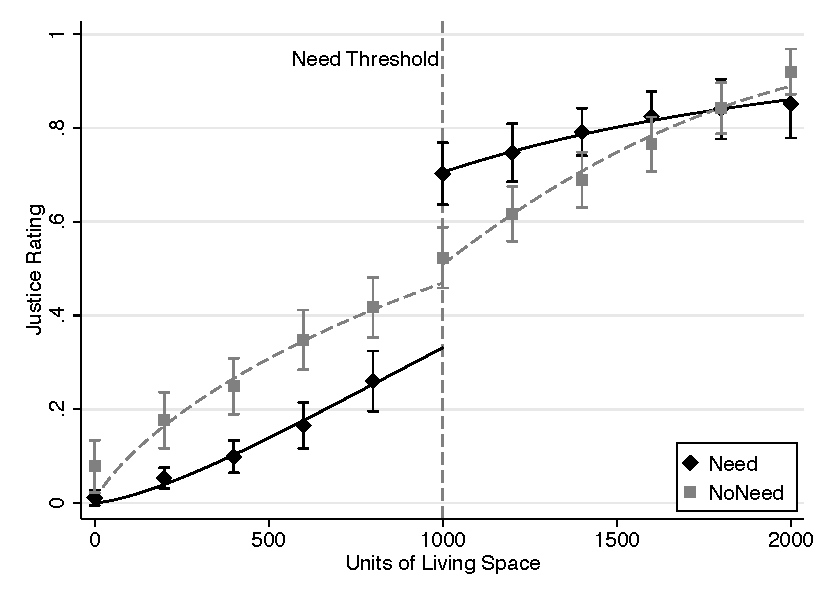
\includegraphics{figures/figure_1.pdf}
   \begin{minipage}{\linewidth}
      \footnotesize
      \textit{The figure shows the mean justice ratings for $x=\{0,200,\ldots,2000\}$ units of living space on a $[0,1]$ scale and the respective $90\%$ confidence intervals of $n=52$ ($n=57$) subjects in the global rating task of the Need (NoNeed) treatment. The solid (dashed) line represents the Weibull fit to the $m=572$ ($m=627$) data points with $r=1000$ as reference point.}
   \end{minipage}
   \caption{Mean Justice Ratings in the Global Rating Task}
   \label{fig:global_ratings_full}
\end{figure}


%%%%%%%%%%%%%%%%%%%%%%%
% MEAN RATINGS GLOBAL %
%%%%%%%%%%%%%%%%%%%%%%%
\subsection{Mean Justice Ratings in the Global Rating Task}\label{sec:global}
We start the analysis of the full sample with the subjects' mean justice ratings in the global rating task.
Figure \ref{fig:global_ratings_full} shows the subjects' mean justice ratings in the global rating task by treatment and stimulus.
The respective means, standard errors, and $t$ tests are stated in Table \ref{tab:global_ratings_full}.

\begin{table}[ht!]
   \centering
   \caption{Mean Justice Ratings in the Global Rating Task by Treatment}\label{tab:global_ratings_full}
   \begin{tabular}{rd{1.3}d{1.3}cd{1.3}d{1.3}cd{2.3}d{1.3}d{1.3}}                         \\[-0.5ex]\hline
           & \multicolumn{2}{c}{Need}   &   & \multicolumn{2}{c}{NoNeed}   &   & \multicolumn{3}{c}{$t$ test}   \\\cline{2-3}\cline{5-6}\cline{8-10}
   Units   & \multicolumn{1}{c}{Mean}   & \multicolumn{1}{c}{SE}   &   & \multicolumn{1}{c}{Mean}   & \multicolumn{1}{c}{SE}   &   & \multicolumn{1}{c}{Mean Diff.}   & \multicolumn{1}{c}{SE}   & \multicolumn{1}{c}{$p$ Value}   \\\hline\hline
      0    & 0.011   & 0.009   &   & 0.078   & 0.034   &   & -0.067   & 0.036   & 0.070   \\
    200    & 0.053   & 0.013   &   & 0.176   & 0.036   &   & -0.123   & 0.039   & 0.002   \\
    400    & 0.099   & 0.021   &   & 0.249   & 0.036   &   & -0.150   & 0.042   & 0.000   \\
    600    & 0.165   & 0.029   &   & 0.348   & 0.038   &   & -0.182   & 0.049   & 0.000   \\
    800    & 0.260   & 0.038   &   & 0.417   & 0.038   &   & -0.157   & 0.054   & 0.005   \\\hline
   1000    & 0.702   & 0.040   &   & 0.523   & 0.039   &   &  0.179   & 0.055   & 0.002   \\
   1200    & 0.747   & 0.037   &   & 0.617   & 0.035   &   &  0.130   & 0.051   & 0.012   \\
   1400    & 0.792   & 0.030   &   & 0.689   & 0.035   &   &  0.102   & 0.047   & 0.032   \\
   1600    & 0.824   & 0.032   &   & 0.765   & 0.035   &   &  0.059   & 0.048   & 0.223   \\
   1800    & 0.840   & 0.038   &   & 0.842   & 0.032   &   & -0.002   & 0.050   & 0.973   \\
   2000    & 0.852   & 0.044   &   & 0.920   & 0.029   &   & -0.068   & 0.051   & 0.186   \\\hline
   \multicolumn{10}{p{13cm}}{\footnotesize\textit{The table shows the mean justice ratings of $x=\{0,200,\ldots,2000\}$ units of living space on a $[0,1]$ scale and the respective standard errors of $n=52$ ($n=57$) subjects in the global rating task of the Need (NoNeed) treatment, and the results of a $t$ test (mean differences, standard errors, $p$ values) on the mean difference (Welch test). Positive (negative) mean differences mean that the respective number of units of living space was rated as more (less) just in the Need treatment than in the NoNeed treatment.}}
   \end{tabular}
\end{table}

We also fit a Weibull distribution $J(c)=1-\exp(-\lambda c^k)$ to the data using STATA's nonlinear-regression package.
The Weibull is often used in psychometric research.
Note that $k$ is called the ``shape parameter''.
If $k<1$, the mean justice rating increases at a \textit{decreasing} rate.
If $k=1$, the Weibull reduces to an exponential distribution and the justice rating increases at a \textit{constant} rate.
In both cases $k\le 1$, the JEF is concave.
If $k>1$, the justice rating first increases at an \textit{increasing} rate up to an inflection point.
Hence it is convex below and concave above the inflection point.
$\lambda$ is called the ``scale parameter'' and gives the dispersion of justice ratings.
In the regression, we also interact the parameters of the Weibull distribution ($\lambda$, $k$) with a dummy variable $D$ for $x\ge 1000$ units.
The results are displayed in Table \ref{tab:weibull_full} and are additionally shown in Figure \ref{fig:global_ratings_full}.
The dashed line represents the Weibull fit for NoNeed and the solid line for Need.
The lines represent the regressions with reference point $r=1000$ units since this gives a better fit in both treatments.

\begin{table}[ht!]
   \centering
   \caption{Fitted Parameters of the Weibull Distribution}\label{tab:weibull_full}
   \begin{tabular}{ld{2.6}d{3.6}cd{2.6}d{3.6}}                                                                 \\[-0.5ex]\hline
                           & \multicolumn{2}{c}{Need}   &   & \multicolumn{2}{c}{NoNeed}                       \\\cline{2-3}\cline{5-6}
   Parameter               & \multicolumn{1}{c}{$r=0$}   & \multicolumn{1}{c}{$r=1000$}   &   & \multicolumn{1}{c}{$r=0$}   & \multicolumn{1}{c}{$r=1000$}   \\\hline\hline
   $\lambda_0$             &   0.00087^{***}   &   0.00053^{***}   &   &   0.00084^{***}   &   0.00056^{***}   \\
		                   &  (0.00002)        &  (0.00016)        &   &  (0.00002)        &  (0.00015)        \\
   $\lambda_1\times D$     &                   &   0.00081^{***}   &   &                   &   0.00025^{*}     \\
                           &                   &  (0.00027)        &   &                   &  (0.00015)        \\
   $k_0$                   &   2.00423^{***}   &   1.43208^{***}   &   &   1.25965^{***}   &   0.78351^{***}   \\
                           &  (0.12243)        &  (0.39590)        &   &  (0.08312)        &  (0.17109)        \\[0.5ex]
   H0: $p(k_0\le 1)$       &   0.000           &   0.138           &   &   0.001           &   0.897           \\[0.5ex]
   $k_1\times D$           &                   &  -0.74159^{*}     &   &                   &   0.84806^{***}   \\
                           &                   &  (0.43163)        &   &                   &  (0.26140)        \\[0.5ex] 
   H0: $p(k_0+k_1\le 1)$   &                   &   0.964           &   &                   &   0.001           \\[0.5ex]\hline
   $n$                     & 572               & 572               &   & 627               & 627               \\
   $\bar{R}^2$             &   0.8542          &   0.8704          &   &   0.8220          &   0.8242          \\
   $RMSE$                  &   0.2434          &   0.2296          &   &   0.2678          &   0.2661          \\\hline
   \multicolumn{6}{p{13cm}}{\footnotesize\textit{The table shows the results of fitting a Weibull distribution to the subjects' justice ratings in the global rating task using nonlinear OLS by treatment. $D=0\,(1)$ for $x<(\ge)1000$ units of living space. First row: means, second row: standard errors. $^{***}p\le0.01$, $^{**}p\le0.05$, $^{*}p\le0.10$. $m=574$ ($m=627$).}}
   \end{tabular}
\end{table}

Figure \ref{fig:global_ratings_full} suggests that the mean justice ratings in the NoNeed treatment initially increase with decreasing rate.
At $r=1000$ units, there is surprisingly a small ``jump'', although no reference point was given.
The ``jump'' indicates that at least some subjects perceived $1000$ units of living space---which is half the maximum possible---as some kind of natural reference point.
We will come back to this observation in Subsection \ref{sec:individual}, where we analyze the individual justice ratings.

For endowments of at least $1000$ units, the mean justice rating increases again at a decreasing rate.
According to the Weibull regression in Table \ref{tab:weibull_full} (NoNeed, $r=1000$), we cannot reject the null hypothesis of concavity ($k_0\le 0$) for endowments with living space smaller than $1000$ units.
For endowments at and above $1000$ units, the null hypothesis ($k_0+k_1\le 1$) is rejected.
However, the inflection point is at $690$ units\footnote{The Maple output for computing the derivatives of $J(c)$ is available from the authors on request.}, this is, below the relevant range of $[1000,2000]$.
Overall, in the NoNeed treatment, the JEF consists of two concave segments.

Turning to the Need treatment, the solid line in Figure \ref{fig:global_ratings_full} exhibits a convex shape below, a ``jump'' of about $35$ percentage points at, and a concave shape above the need threshold.
The inflection point is at $817$ units of living space, this is, just below the need threshold.
However, according to Table \ref{tab:weibull_full} (NoNeed, $r=1000$) the null hypothesis of concavity for endowments with living space smaller than $1000$ units is just barely not rejected ($p=0.138$).
For endowments in the range $[1000,2000]$, concavity is clearly not rejected ($p=0.964$).
Overall, in the Need treatment, the JEF tends to be convex below the need threshold and is concave above.

Thus, Figure \ref{fig:global_ratings_full} displays a striking difference between the Need and the NoNeed treatment.
According to Table \ref{tab:global_ratings_full}, mean justice ratings are significantly lower (higher) in the Need than in the NoNeed treatment (except for $0$ and for $1600$ or more units of living space).

In Appendix \ref{sec:app_conditional_absolute}, Figure \ref{fig:global_ratings_conditional} as well as Tables \ref{tab:global_ratings_conditional} and \ref{tab:weibull_conditional} display the results of performing the same analysis with the conditional sample.
Although the fit of the Weibull regression improves a bit when the subjects with non-monotonic responses are excluded, the results remain qualitatively unchanged.
In particular, the aggregated JEF still tends to be convex below and is concave above the need threshold in the Need treatment.


%%%%%%%%%%%%%%%%%%%%%%%%%
% MEAN RATINGS RELATIVE %
%%%%%%%%%%%%%%%%%%%%%%%%%
\subsection{Mean Justice Ratings in the Relative Rating Task}\label{sec:relative}
As noted in Subsection \ref{sec:remarks}, we conducted the relative rating task in order to address the concern that bunching at extreme values may bias subjects' justice ratings in the absolute rating task.
Again, we use the full sample.
We show the results for the conditional sample, only including subjects who exhibit weakly monotonic increasing justice ratings in Appendix \ref{sec:app_conditional_relative}.

Figure \ref{fig:relative_ratings_full} depicts the results of the relative rating task, which provided subjects for every pair-wise comparison with a separate rating scale.
Means, standard errors and $t$ tests are stated in Table \ref{tab:relative_ratings_full}.

\begin{figure}[h]
   \centering
   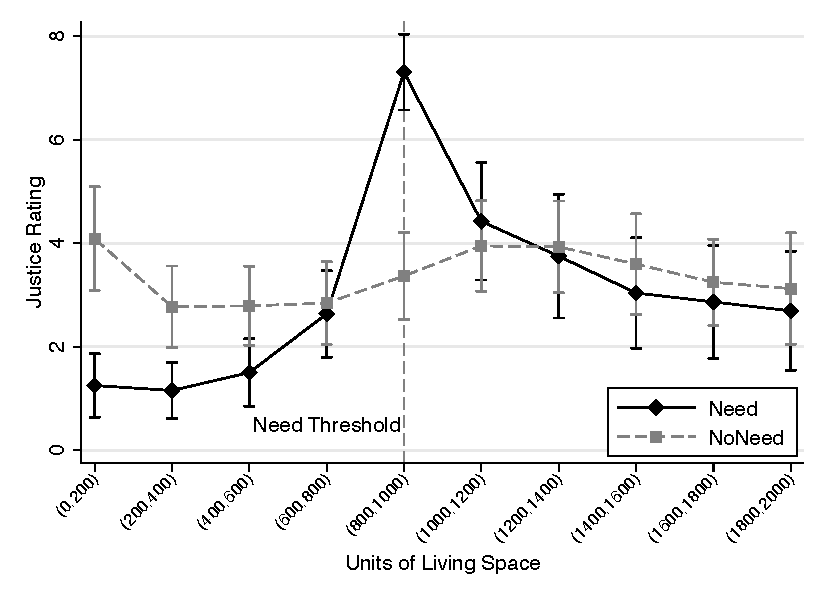
\includegraphics{figures/figure_2.pdf}
   \begin{minipage}{\linewidth}
      \footnotesize
      \textit{The figure shows the mean justice ratings of comparing two adjacent endowments with $\{(0,200),(200,400),\ldots,(1800,2000)\}$ units of living space on a $[-11,+11]$ Likert scale and the respective $90\%$ confidence intervals of $n=52$ ($n=57$) subjects in the relative rating task of the Need (NoNeed) treatment. Positive (negative) numbers indicate that the larger endowment was rated as more (less) just than the smaller endowment.}
   \end{minipage}
   \caption{Mean Justice Ratings in the Relative Rating Task}
   \label{fig:relative_ratings_full}
\end{figure}

\begin{table}[ht!]
   \centering
   \caption{Mean Justice Ratings in the Relative Rating Task by Treatment}\label{tab:relative_ratings_full}
   \begin{tabular}{ld{1.2}d{1.2}cd{1.2}d{1.2}cd{1.2}d{1.2}d{1.2}}                           \\[-0.5ex]\hline
                   & \multicolumn{2}{c}{Need}   &   & \multicolumn{2}{c}{NoNeed}   &   & \multicolumn{3}{c}{$t$ Test}   \\\cline{2-3}\cline{5-6}\cline{8-10}
   Units           & \multicolumn{1}{c}{Mean}   & \multicolumn{1}{c}{SE}   &   & \multicolumn{1}{c}{Mean}   & \multicolumn{1}{c}{SE}   &   & \multicolumn{1}{c}{Diff.}   & \multicolumn{1}{c}{SE}   & \multicolumn{1}{c}{$p$ Value}   \\\hline\hline
      $(0,200)$    & 1.25   & 0.37   &   & 4.09   & 0.60   &   & -2.84   & 0.72   & 0.000   \\
    $(200,400)$    & 1.15   & 0.33   &   & 2.77   & 0.47   &   & -1.62   & 0.58   & 0.007   \\
    $(400,600)$    & 1.50   & 0.39   &   & 2.79   & 0.46   &   & -1.29   & 0.61   & 0.036   \\
    $(600,800)$    & 2.63   & 0.50   &   & 2.84   & 0.48   &   & -0.21   & 0.69   & 0.765   \\
    $(800,1000)$   & 7.31   & 0.44   &   & 3.37   & 0.50   &   &  3.94   & 0.67   & 0.000   \\\hline
   $(1000,1200)$   & 4.42   & 0.68   &   & 3.95   & 0.52   &   &  0.48   & 0.85   & 0.576   \\
   $(1200,1400)$   & 3.75   & 0.71   &   & 3.93   & 0.53   &   & -0.18   & 0.88   & 0.838   \\
   $(1400,1600)$   & 3.04   & 0.64   &   & 3.60   & 0.58   &   & -0.56   & 0.88   & 0.518   \\
   $(1600,1800)$   & 2.87   & 0.65   &   & 3.24   & 0.50   &   & -0.38   & 0.81   & 0.641   \\
   $(1800,2000)$   & 2.69   & 0.69   &   & 3.12   & 0.64   &   & -0.43   & 0.94   & 0.648   \\\hline
   \multicolumn{10}{p{12.5cm}}{\footnotesize\textit{The table shows the mean justice ratings comparing two adjacent endowments with $\{(0,200),(200,400),\ldots,(1800,2000)\}$ units of living space on a $[-11,+11]$ Likert scale of $n=52$ ($n=57$) subjects in the relative rating task of the Need (NoNeed) treatment, and the results of a $t$ test (mean differences, standard errors, $p$ values) on the mean difference (Welch test). Positive (negative) means indicate that the larger endowment was rated as more (less) just than the smaller endowment. Positive (negative) mean differences indicate that the respective comparison was rated as more (less) just in the Need treatment than in the NoNeed treatment.}}
   \end{tabular}
\end{table}

On the whole, Figure \ref{fig:relative_ratings_full} corroborates the results of the absolute rating task.
In the Need treatment, increasing the endowment by $200$ units of living space raises justice ratings only by about $1$ to $2$ points on the Likert scale when the adjustment takes place below the need threshold; it raises justice ratings by about $3$ to $5$ points when above the need threshold; and justice ratings ``jump'' by $7$ points when the need threshold is met exactly.

Relative justice ratings are significantly worse in the Need treatment than in the NoNeed treatment for adjustments below the need threshold (with the exception of ($600,800$) which is insignificant) and better for ($800,1000$); they are identical for adjustments above the need threshold.

In the NoNeed treatment, relative justice ratings meander between slightly below $3$ and above $4$ points.
The drop from $4.09$ ($0,200$) to $2.77$ ($200,400$) points in the beginning is significant ($p\le 0.01$, two-tailed $t$ test), which supports concavity of the JEF for low endowments in the NoNeed treatment.
Using the full instead of the conditional sample does not change the results (see Figure \ref{fig:relative_ratings_conditional} and Table \ref{tab:relative_ratings_conditional} in Appendix \ref{sec:app_conditional_relative}).


%%%%%%%%%%%%%%%%%%%%%%
% INDIVIDUAL RATINGS %
%%%%%%%%%%%%%%%%%%%%%%
\subsection{Individual Justice Ratings}\label{sec:individual}
\noindent In this subsection, we analyze the individual justice ratings in the global rating task for the full sample of $52$ ($57$) subjects with valid observations in the Need (NoNeed) treatment.
More precisely, we try to identify different justice principles according to subjects' individual-specific patterns of justice ratings and how they responded to the need threshold, in particular.

\begin{landscape}
\begin{figure}
   \centering
   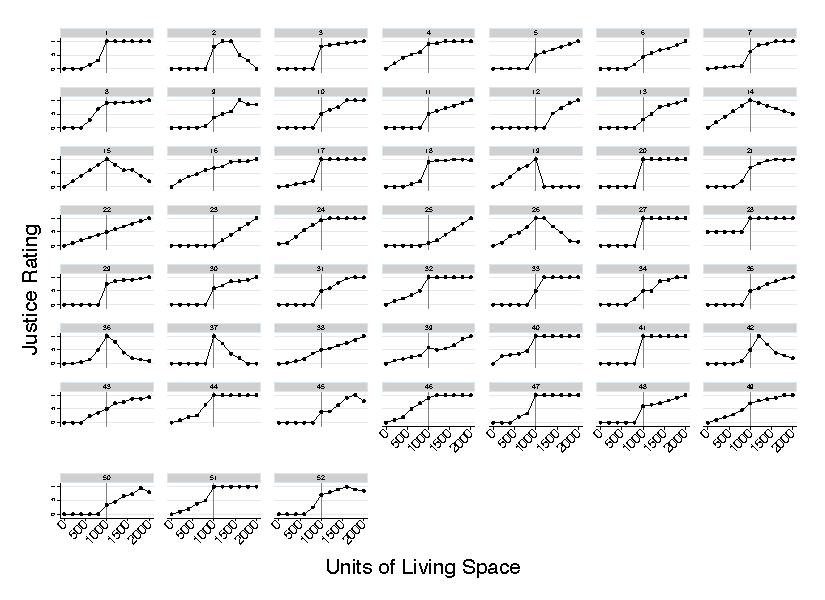
\includegraphics{figures/figure_3.pdf}
   \begin{minipage}{0.7\linewidth}
      \footnotesize
      \textit{The figure shows a connected line graph of the individual justice ratings of endowments with $\{0,200,\ldots,2000\}$ units of living space on a $[0,1]$ scale of $n=52$ subjects in the global rating task of the Need treatment. The need threshold at $x=1000$ units is marked by a horizontal line.}
   \end{minipage}
   \caption{Individual Justice Ratings in the Global Rating Task of the Need treatment}
   \label{fig:individual_need}
\end{figure}
\end{landscape}

\begin{landscape}
\begin{figure}
   \centering
   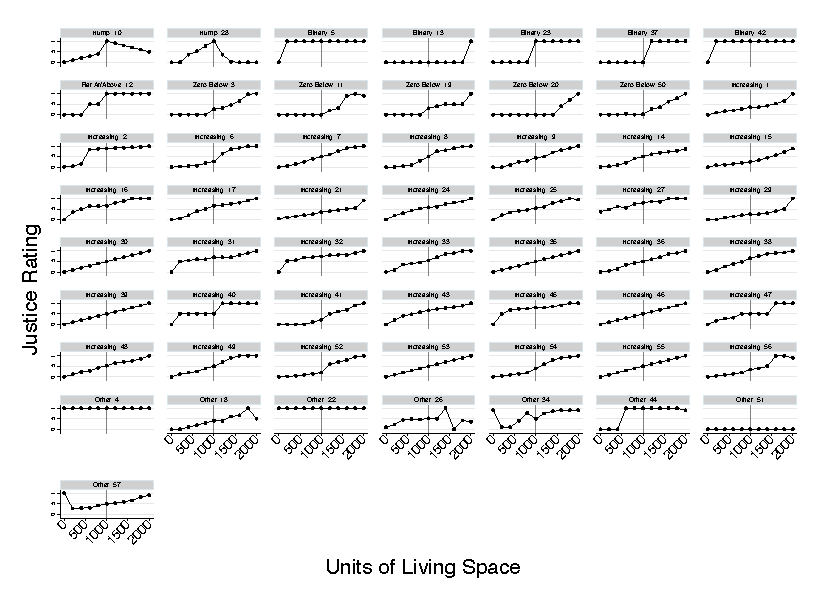
\includegraphics{figures/figure_4.pdf}
   \begin{minipage}{0.7\linewidth}
      \footnotesize
      \textit{The figure shows a connected line graph of the individual justice ratings of endowments with $\{0,200,\ldots,2000\}$ units of living space on a $[0,1]$ scale of $n=57$ subjects in the global rating task of the NoNeed treatment.}
   \end{minipage}
   \caption{Individual Justice Ratings in the Global Rating Task of the NoNeed treatment}
   \label{fig:individual_noneed}
\end{figure}
\end{landscape}

Figure \ref{fig:individual_need} shows a connected line graph of the individual justice ratings of endowments by subject identification number (ID) in the Need treatment.
The figure reveals that there is a lot of heterogeneity with respect to subjects' response patterns.
In Table \ref{tab:individual}, we assign each subject to one of five justice types by graphical inspection.
The individual classification can be taken from Table \ref{tab:classification} in the Appendix.
In principle, a formal estimation of the individual justice evaluation function with the $11$ data points each would also be possible.
However, non-monotonous, partially flat, or even binary responses to the stimuli would cause statistical difficulties.
Therefore, we leave it at a ``normative'' visual assessment of the JEF types and freely acknowledge that this \textit{modus operandi} is, to some extent, subjective.
However, the classification can be easily checked using the two figures and Table \ref{tab:classification}.

\begin{table}[ht!]
   \centering
   \caption{Types of Justice Ratings}\label{tab:individual}
   {\normalsize\small
   \begin{tabular}{lccccccl}\hline\\[-2.5ex]
   Type             & \multicolumn{5}{c}{Number}   &   & Justice Principle                                           \\\cline{2-6}\\[-2.5ex]
                    & \multicolumn{2}{c}{Need}     &   & \multicolumn{2}{c}{NoNeed}   &   &                          \\\hline\hline
   Hump-Shaped      &  8   &  (15.4\%)             &   &  2   &   (3.5\%)             &   & ``Strict''               \\
                    &      &                       &   &      &                       &   & Sufficientarianism       \\[1ex]
   Binary           &  4   &   (7.7\%)             &   &  6   &  (10.5\%)             &   & ``Qualitative''          \\
                    &      &                       &   &      &                       &   & Sufficientarianism       \\[1ex]
   Flat at/above    &  8   &  (15.4\%)             &   &  5   &   (8.8\%)             &   & ``Quantitative''         \\
   Need Threshold   &      &                       &   &      &                       &   & Sufficientarianism       \\[1ex]
   Zero below       & 16   &  (30.8\%)             &   &  6   &  (10.5\%)             &   & ``Strict''               \\
   Need Threshold   &      &                       &   &      &                       &   & Prioritarianism          \\[1ex]
   Increasing       & 16   &  (30.8\%)             &   & 32   &  (56.1\%)             &   & Utilitarianism           \\[1ex]
   Other            & ---  &                       &   &  6   &  (10.5\%)             &   & e.\,g.,~Egalitarianism   \\[0.5ex]\hline
                    & 52   & (100.0\%)             &   & 57   & (100.0\%)             &   &                          \\\hline
   \end{tabular}
   }
\end{table}

In the Need treatment, there are $8$ subjects ($15.4\%$) who exhibit a \textit{hump-shaped} JEF which violates the monotonicity assumption.
The hump-shaped JEF reaches its maximum at or slightly above $1000$ units and then drops sharply.
Since we clearly told subjects in the instructions that more living space means higher household utility and that spending on living space does not involve opportunity costs, this result is somewhat surprising.
Either these subjects did not understand the instructions correctly or they actually believed that it is unfair to have more than is necessary.
Perhaps, environmental concerns played a role.
The latter reasoning would suggest an attitude halfway compatible with a strict account of sufficientarianism that ``punishes'' oversupply.
Only $4$ subjects ($7.7\%$) exhibit a \textit{binary} JEF that is $0$ ($0.5$ in one case) for endowments below and $1$ for endowments at and above the need threshold.
The binary shape of the JEF could be viewed as a qualitative account of sufficientarianism that only distinguishes between unjust insufficient and just sufficient endowments.
The JEFs of $8$ subjects ($15.4\%$) increase below and reach the maximum of $1$ at the need threshold.
They are \textit{flat at and above the need threshold}.
This shape of the JEF is compatible with a quantitative account of sufficientarianism that is able to differentiate between different degrees of unjust insufficiency.

$16$ subjects ($30.8\%$) rated endowments below the need threshold as completely unfair and only increased their justice ratings at and above the need threshold.
A JEF that is \textit{zero below the need threshold} can be interpreted as a strict account of prioritarianism that regards the need threshold as absolute.
In demand theory, a similar idea is covered by the Stone-Geary utility function \citep{geary_note_1950,stone_linear_1954}, which assumes that the minimum consumption level is indispensable to life and that only consumption levels exceeding them generate utility.\footnote{For an experimental investigation of need thresholds in risky scenarios see \citet{diederich_need_2020}.}

The \textit{utilitarian} type increases her justice rating throughout ($16$ subjects, $30.8\%$).
However, Figure \ref{fig:individual_need} shows different shapes of the JEF, which are concave, convex, sigmoid, or almost linear in the endowment with living space.
Note that we were a bit more generous in this category, including as utilitarian also those $3$ subjects whose JEF did not consistently increase (subject numbers $9$, $39$, and $52$).

Overall, in the Need treatment, we find that about one-third of individual justice ratings are compatible with sufficientarianism, priortarianism, and utilitarianism, respectively.
We looked for differences between the justice types with regard to sociodemographics, living conditions, and political attitudes but found no significant effects.

Analogously, Figure \ref{fig:individual_noneed} shows a connected line graph of the individual justice ratings of endowments with units of living space by subject identification number (ID) in the NoNeed treatment.
The respective column in Table \ref{tab:individual} summarizes the type assignment, and the individual classification can be taken from Table \ref{tab:classification} in the Appendix.
Although there was no communicated need threshold in NoNeed, subjects could nevertheless have assumed that people need some minimum endowment with living space in their justice ratings.
In fact, the absolute majority ($32$ subjects, $56.1\%$) of the JEFs have a strong monotonically increasing shape (with a maximum of one non-increasing evaluation being allowed in order to account for errors), so it is clearly \textit{utilitarian}.
A proportion test clearly rejects the null hypothesis that Need and NoNeed treatments give rise to the same proportion of utilitarian justice evaluations ($z=2.67$, $p=0.008$).

In NoNeed, we find only $2$ subjects with \textit{hump-shaped} JEFs with the maximum justice at $1000$ units of living space.
$6$ subjects exhibit a \textit{binary} JEF, which jumps from $0$ to $1$ at some value of units of living space on the interval $[200,1800]$.
Further $5$ subjects can be classified as quantitative sufficientarians because their JEF is \textit{flat at and above the need threshold}.
Altogether, there are $13$ sufficientarian justice evaluations.
A proportion test shows that sufficientarian justice evaluations are almost twice as common among subjects in the Need treatment as in the NoNeed treatment ($z=1.98$, $p=0.048$).
There are only $6$ JEFs exhibiting a ``prioritarian'' shape (assuming \textit{zero below} some assumed \textit{need threshold} greater than $400$ units).
Thus, the proportion of prioritarians is almost three times bigger in Need as in NoNeed ($z=2.63$, $p=0.009$).
In NoNeed, we also observe $2$ subjects who rated all endowments as perfectly just, which is compatible with a comparative egalitarian justice attitude; $1$ subject rated all endowments as perfectly unjust, which is, perhaps, a ``negative'' egalitarian justice attitude; and $3$ subjects stated irregular JEFs.

To summarize this subsection, it can be stated that the introduction of an explicit need threshold leads to a statistically significant change in the justice evaluation of endowments with living space at the individual level.
The heterogeneity of justice attitudes not only increases with the introduction of the need threshold but also changes in the direction of less utilitarianism and more prioritarianism and sufficientarianism.


%%%%%%%%%%%%%%
% CONCLUSION %
%%%%%%%%%%%%%%
\section{Conclusion}\label{sec:conclusion}


%%%%%%%%%%%%%%%%
% BIBLIOGRAPHY %
%%%%%%%%%%%%%%%%
\newpage
\bibliographystyle{elsarticle-harv}
\bibliography{references.bib}


%%%%%%%%%%%%
% APPENDIX %
%%%%%%%%%%%%
\newpage
\appendix
\section{Mean Justice Ratings in the Global Rating Task: Conditional Sample}\label{sec:app_conditional_absolute}
\begin{figure}[ht!]
   \centering
   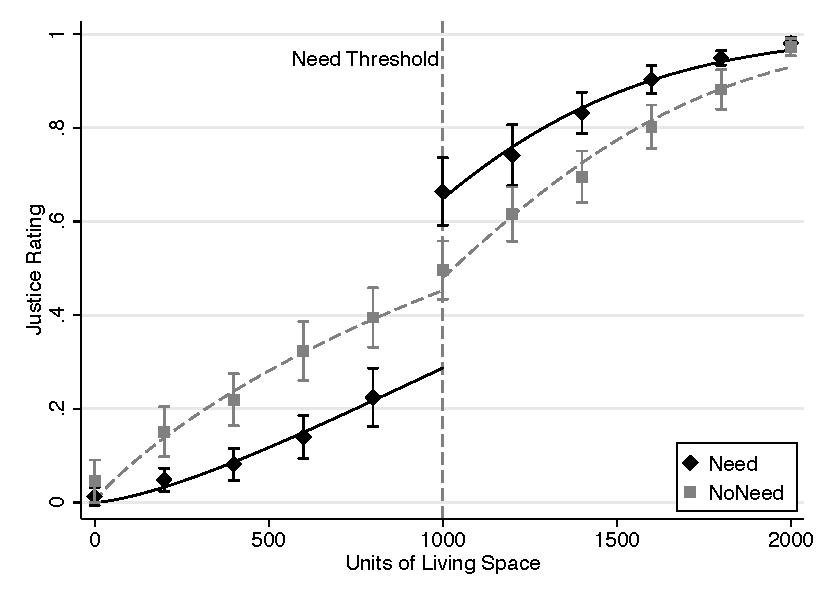
\includegraphics{figures/figure_5.pdf}
   \begin{minipage}{\linewidth}
      \footnotesize
      \textit{The figure shows the mean justice ratings for $x=\{0,200,\ldots,2000\}$ units of living space on a $[0,1]$ scale and the respective $90\%$ confidence intervals of $n=44$ ($n=51$) subjects in the global rating task of the Need (NoNeed) treatment. The solid (dashed) line represents the Weibull fit to the $m=484$ ($m=561$) data points with $r=1000$ as reference point.}
   \end{minipage}
   \caption{Mean Justice Ratings in the Global Rating Task: Conditional Sample}
   \label{fig:global_ratings_conditional}
\end{figure}

\clearpage
\begin{table}[ht!]
   \centering
   \caption{Mean Justice Ratings in the Global Rating Task by Treatment: Conditional Sample}\label{tab:global_ratings_conditional}
   \begin{tabular}{rd{1.3}d{1.3}cd{1.3}d{1.3}cd{2.3}d{1.3}d{1.3}}                         \\[-0.5ex]\hline
           & \multicolumn{2}{c}{Need}   &   & \multicolumn{2}{c}{NoNeed}   &   & \multicolumn{3}{c}{$t$ test}   \\\cline{2-3}\cline{5-6}\cline{8-10}
   Units   & \multicolumn{1}{c}{Mean}   & \multicolumn{1}{c}{SE}   &   & \multicolumn{1}{c}{Mean}   & \multicolumn{1}{c}{SE}   &   & \multicolumn{1}{c}{Mean Diff.}   & \multicolumn{1}{c}{SE}   & \multicolumn{1}{c}{$p$ Value}   \\\hline\hline
      0    & 0.013   & 0.011   &   & 0.046   & 0.027   &   & -0.033   & 0.031   & 0.291   \\
    200    & 0.048   & 0.014   &   & 0.151   & 0.032   &   & -0.103   & 0.037   & 0.007   \\
    400    & 0.081   & 0.020   &   & 0.219   & 0.033   &   & -0.138   & 0.040   & 0.001   \\
    600    & 0.140   & 0.027   &   & 0.324   & 0.038   &   & -0.184   & 0.048   & 0.000   \\
    800    & 0.224   & 0.037   &   & 0.395   & 0.040   &   & -0.171   & 0.053   & 0.002   \\\hline
   1000    & 0.664   & 0.043   &   & 0.496   & 0.037   &   &  0.169   & 0.057   & 0.004   \\
   1200    & 0.742   & 0.039   &   & 0.616   & 0.026   &   &  0.126   & 0.052   & 0.017   \\
   1400    & 0.832   & 0.026   &   & 0.695   & 0.033   &   &  0.136   & 0.043   & 0.002   \\
   1600    & 0.903   & 0.018   &   & 0.802   & 0.028   &   &  0.101   & 0.034   & 0.004   \\
   1800    & 0.949   & 0.009   &   & 0.882   & 0.025   &   &  0.067   & 0.028   & 0.020   \\
   2000    & 0.980   & 0.008   &   & 0.972   & 0.011   &   &  0.008   & 0.014   & 0.567   \\\hline
   \multicolumn{10}{p{13cm}}{\footnotesize\textit{The table shows the mean justice ratings of $x=\{0,200,\ldots,2000\}$ units of living space on a $[0,1]$ scale and the respective standard errors of $n=44$ ($n=51$) subjects in the global rating task of the Need (NoNeed) treatment, and the results of a $t$ test (mean differences, standard errors, $p$ values) on the mean difference (Welch test). Positive (negative) mean differences indicate that the respective number of units of living space was rated as more (less) just in the Need treatment than in the NoNeed treatment.}}
   \end{tabular}
\end{table}

\clearpage
\begin{table}[ht!]
   \centering
   \caption{Fitted Parameters of the Weibull Distribution: Conditional Sample}\label{tab:weibull_conditional}
   \begin{tabular}{ld{2.8}d{2.6}cd{2.6}d{2.6}}                                                                 \\[-0.5ex]\hline
                           & \multicolumn{2}{c}{Need}  &  & \multicolumn{2}{c}{NoNeed} \\ \cline{2-3}\cline{5-6}
   Parameter               & \multicolumn{1}{c}{$r=0$}   & \multicolumn{1}{c}{$r=1000$}   &   & \multicolumn{1}{c}{$r=0$}   & \multicolumn{1}{c}{$r=1000$}   \\ \hline\hline
   $\lambda_0$             &   0.00091^{***}   &   0.00047^{***}   &   &   0.00085^{***}   &   0.00056^{***}   \\
                           &  (0.00001)        &  (0.00015)        &   &  (0.00002)        &  (0.00013)        \\[1ex]
   $\lambda_1\times D$     &                   &   0.00056^{***}   &   &                   &   0.00025^{*}     \\
                           &                   &  (0.00015)        &   &                   &  (0.00013)        \\[1ex]
   $k_0$                   &   2.84639^{***}   &   1.44034^{***}   &   &   1.50106^{***}   &   0.87042^{***}   \\
                           &  (0.15670)        &  (0.37578)        &   &  (0.08633)        &  (0.17041)        \\[1ex]
   H0: $p(k_0\le 1)$       &   0.000           &   0.242           &   &   0.000           &   0.447           \\[1ex]
   $k_1\times D$           &                   &   0.25428         &   &                   &   1.15519^{***}   \\
                           &                   &  (0.42271)        &   &                   &  (0.25941)        \\[1ex]
   H0: $p(k_0+k_1\le 1)$   &                   &   0.000           &   &                   &   0.000           \\\hline
   $n$                     & 484               & 484               &   & 561               & 561               \\
   $\bar{R}^2$             &   0.9252          &   0.9322          &   &   0.8692          &   0.8729          \\
   $RMSE$                  &   0.1799          &   0.1712          &   &   0.2276          &   0.2243          \\\hline
   \multicolumn{6}{p{13cm}}{\footnotesize\textit{The table shows the results of fitting a Weibull distribution to the subjects' justice ratings in the global rating task using nonlinear OLS by treatment. $D=0(1)$ for $x<(\ge )1000$ units of living space. First row: means, second row: standard errors. $^{***}p\le 0.01$, $^{**}p\le 0.05$, $^{*}p\le 0.10$. $m=484$ ($m=561$).}}
   \end{tabular}
\end{table}

\clearpage
\section{Mean Justice Ratings in the Relative Rating Task: Conditional Sample}\label{sec:app_conditional_relative}
\begin{figure}[ht!]
   \centering
   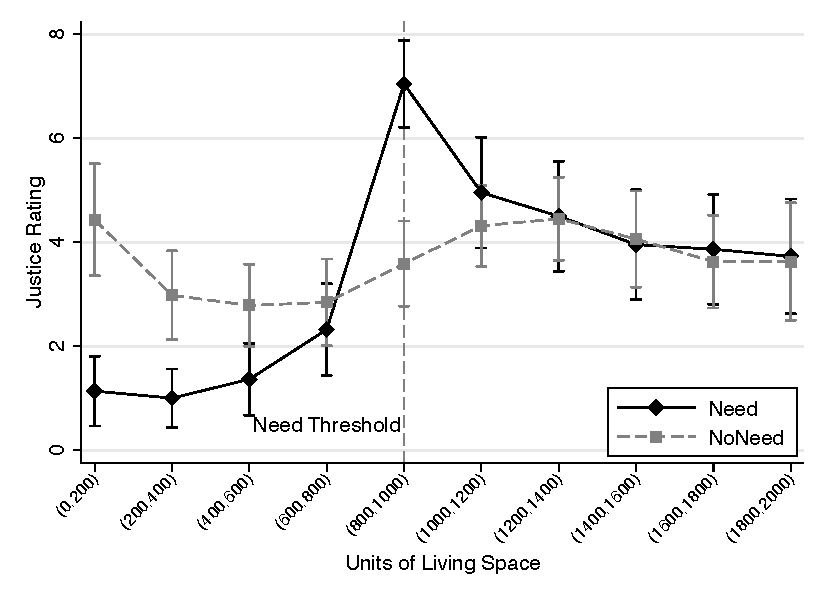
\includegraphics{figures/figure_6.pdf}
   \begin{minipage}{\linewidth}
      \footnotesize
      \textit{The figure shows the mean justice ratings of comparing two adjacent endowments with $\{(0,200),(200,400),\ldots,(1800,2000)\}$ units of living space on a $[-11,+11]$ Likert scale and the respective $90\%$ confidence intervals of $n=44$ ($n=51$) subjects in the relative rating task of the Need (NoNeed) treatment. Positive (negative) numbers indicate that the larger endowment was rated as more (less) just than the smaller endowment.}
   \end{minipage}
   \caption{Mean Justice Ratings in the Relative Rating Task: Conditional Sample}
   \label{fig:relative_ratings_conditional}
\end{figure}

\clearpage
\begin{table}[ht!]
   \centering
   \caption{Mean Justice Ratings in the Relative Rating Task by Treatment: Conditional Sample}\label{tab:relative_ratings_conditional}
   \begin{tabular}{ld{1.2}d{1.2}cd{1.2}d{1.2}cd{2.2}d{1.2}d{1.3}}                         \\[-0.5ex]\hline
                 & \multicolumn{2}{c}{Need}   &   & \multicolumn{2}{c}{NoNeed}   &   & \multicolumn{3}{c}{t Test}   \\\cline{2-3}\cline{5-6}\cline{8-10}
   Units         & \multicolumn{1}{c}{Mean}   & \multicolumn{1}{c}{SE}   &   & \multicolumn{1}{c}{Mean}   & \multicolumn{1}{c}{SE}   &   & \multicolumn{1}{c}{Diff.}   & \multicolumn{1}{c}{SE}   & \multicolumn{1}{c}{$p$ Value}   \\\hline\hline
      (0,200)    & 1.14   & 0.40   &   & 4.43   & 0.64   &   & -3.30   & 0.78   & 0.000   \\
    (200,400)    & 1.00   & 0.33   &   & 2.98   & 0.51   &   & -1.98   & 0.63   & 0.002   \\
    (400,600)    & 1.36   & 0.41   &   & 2.78   & 0.47   &   & -1.42   & 0.64   & 0.028   \\
    (600,800)    & 2.32   & 0.53   &   & 2.84   & 0.50   &   & -0.52   & 0.70   & 0.470   \\
    (800,1000)   & 7.05   & 0.50   &   & 3.59   & 0.49   &   &  3.46   & 0.70   & 0.000   \\\hline
   (1000,1200)   & 4.95   & 0.63   &   & 4.31   & 0.46   &   &  0.64   & 0.77   & 0.409   \\
   (1200,1400)   & 4.50   & 0.63   &   & 4.45   & 0.47   &   &  0.05   & 0.78   & 0.950   \\
   (1400,1600)   & 3.95   & 0.63   &   & 4.06   & 0.55   &   & -0.10   & 0.83   & 0.900   \\
   (1600,1800)   & 3.86   & 0.63   &   & 3.63   & 0.53   &   &  0.24   & 0.82   & 0.774   \\
   (1800,2000)   & 3.73   & 0.66   &   & 3.63   & 0.67   &   &  0.10   & 0.95   & 0.916   \\\hline
   \multicolumn{10}{p{12.5cm}}{\footnotesize\textit{The table shows the mean justice ratings comparing two adjacent endowments with $\{(0,200),(200,400),\ldots,(1800,2000)\}$ units of living space on a $[-11,+11]$ Likert scale of $n=44$ ($n=51$) subjects in the relative rating task of the Need (NoNeed) treatment, and the results of a $t$ test (mean differences, standard errors, $p$ values) on the mean difference (Welch test). Positive (negative) means indicate that the larger endowment was rated as more (less) just than the smaller endowment. Positive (negative) mean differences indicate that the respective comparison was rated as more (less) just in the Need treatment than in the NoNeed treatment.}}
   \end{tabular}
\end{table}

\clearpage
\begin{landscape}
\begin{table}[ht!]
   \centering
   \caption{Individual Classification of Subjects}\label{tab:classification}
   {\normalsize\small
   \begin{tabular}{lclccl}\hline\\[-1.5ex]
      Type             & \multicolumn{2}{c}{Need}                     &   & \multicolumn{2}{c}{NoNeed}                        \\\cline{2-3}\cline{5-6}
                       & Number   & Subject IDs                       &   & Number   & Subject IDs                            \\\hline\hline
      Hump-Shaped      &  8       &  2, 14, 15, 19, 26, 36, 37, 42    &   &  2       &  62, 80                                \\[1ex]
      Binary           &  4       &  20, 27, 28, 41                   &   &  6       &  57, 65, 75, 89, 94, 96                \\[1ex]
      Flat at/above    &  8       &  1, 17, 24, 32, 40, 44, 47, 51    &   &  5       &  64, 92, 99, 101, 108                  \\
      Need Threshold   &          &                                   &   &          &                                        \\[1ex]
      Zero below       & 16       &  3, 5, 10, 11, 12, 13, 23, 25,    &   &  6       &  55, 63, 71, 72, 93, 102               \\
      Need Threshold   &          &  29, 30, 31, 33, 35, 45, 48, 50   &   &          &                                        \\[1ex]
      Increasing       & 16       &  4, 6, 7, 8, 9, 16, 18, 21,       &   & 32       &  53, 54, 58, 59, 60, 61, 66, 67        \\
                       &          &  22, 34, 38, 39, 43, 46, 49, 52   &   &          &  68, 69, 70, 73, 76, 77, 79, 81        \\
                       &          &                                   &   &          &  82, 83, 84, 85, 87, 88, 90, 91        \\
                       &          &                                   &   &          &  95, 97, 98, 100, 104, 105, 106, 107   \\[1ex]
      Other            & ---      &                                   &   &  6       &  56, 74 (Egalitarian)                  \\
                       &          &                                   &   &          &  103 (Neg. Egalitarian)                \\
                       &          &                                   &   &          &  78, 86, 109 (Irregular)               \\\hline
   \end{tabular}}
\end{table}
\end{landscape}

\clearpage
\section{Vignette Texts}\label{sec:app_vignette}
\subsection*{Introduction Screen}
\noindent Welcome to our study,

\noindent In this study on justice, we are interested in your opinions and assessments.
Therefore we will present to you a number of varying scenarios, and we ask you to imagine them as real.
Please take the time to place yourself into the scenarios and to come to your own personal assessment.
In this study, there are no right or wrong answers.

We will assess your evaluations as well as the evaluations of all other participants in this study.
All data will be saved anonymously so that no details can be attributed to any person.
The results of the study will be published.
Thereby they will influence future research and shall be used to inform politics.

\subsection*{Vignette Texts of the Need and NoNeed Treatments}
\textit{Note: The vignette texts of the Need and NoNeed treatments differ only on the information given with regards to needs, which was left out in the NoNeed treatment, as is indicated in the following by square brackets.}

\medskip{}
\noindent Please imagine the following:

\noindent In the region of Bergtal, a new village is going to be established.
It is the task of the Public Housing Association of Bergtal to build housing.

All households in this region want to live in the largest living space possible.
{[}The residents of the region have collectively decided on a minimum amount of living space, under which living a decent life in this community is not possible.{]}
Between the households in the region, there are no noteworthy differences {[}and the minimum amounts are the same for each household: Each household should have $1000$ regional---i.e., common to the region---area units of living space in order to be able to live a decent life.
To have a living space with the equivalent area means for a household to live in close quarters, but it will be just enough to lead a decent life{]}.

There are enough means to be able to build up to $2000$ regional area units of living space for each household.
The Regional Parliament decides how much living space will actually be built for the residents of the new village.
The decision has otherwise no noteworthy consequences.
For the construction of living space, no additional area would be consumed.
The new village will be built in the area of an old village that was abandoned after a fire destroyed the houses.

In its decision, the Regional Parliament wants to take into account how impartial people---like you---judge the justice of different scenarios.
Your task is, therefore, to indicate for each scenario how just you hold the distribution of living space to be.

\subsection*{Task Descriptions of the Need and NoNeed Treatments}
\textit{Note: Participants received two different task descriptions, one for the justice evaluations of the 11 scenarios each for themselves (global rating task) and one for the pairwise evaluations (relative rating task).}

\subsubsection*{Global Rating Task}
The following scenarios differ in how much living space shall be built for each household according to the decision of the Regional Parliament.

Please indicate for each following distribution how just you regard it to be.
$100$ percent means that you judge the distribution to be completely just.
Percentages close to $100$ percent mean that you judge the distribution to be almost completely just.
Percentages far from $100$ percent mean that you judge the distribution to be significantly
less just.
Please familiarize yourself now with each of the given distributions before answering the questions.

\subsubsection*{Relative Rating Task}
On the coming pages, we will present to you each time two differing scenarios. We will ask you furthermore to indicate on a scale from 1 (equally just or unjust) to 11 (much more just) how just you regard each scenario compared to the other one to be.

\end{document}
